\section{Motivation}
Often in a problem being tackled with Machine Learning (ML) techniques one of the most important part of the solving process is the algorithm selection. Each algorithm has a specific bias which makes it more suitable for some classes of problems than others \cite{Lorena2022}. 

It is desirable, then, that we may have a way of measuring the relationship of the performance of a given algorithm in a problem with the problem's characteristics, since knowing which data is easy or difficult for a given model to classify is useful in the way that we may make changes to the original model.

\cite{Munoz2018} has introduced a methodology called Instance Space Analysis (ISA), a novel way of performance evaluation and algorithm selection in classifiers by mapping the statistical properties of an instance (an entire dataset) into how difficult the instance is for the classification algorithm to perform. Further, in \cite{Lorena2022}, the methodology has been modified to have a more fine-grained analysis, with the instance being reduced to an individual observation in a classification dataset.

Given this, we can map each observation into a hardness level . One type of model that may give us new information from this data is a Generative Adversarial Network (GAN) architecture as defined by \cite{Goodfellow2014}. This architecture is based on a zero-sum game, with a generator network trying to create data matching the original data and a discriminator network trying to discern between the original data and the generated data. 

Using this, we can use the trained generator to create data with specific hardness levels and set a difficulty of classification for an entire dataset. We can use this to verify how the original model behaves with data with a given difficulty profile or to challenge the model.

\section{Objective}

This work's objective lies in providing a framework for data generation based on the relationship between instance hardness and classification performance using the GAN architecture and monitor the original model's behaviour using the generated data. 

\section{Scope}

The scope of this work will be limited to exploring a GAN implementation for the generation of data, creating a Generator and a Discriminator.  The modelling will be made entirely using Python, with the PyTorch \cite{paszke2019pytorch} framework. PyHard \cite{Lorena2022} will be used for reproducing the ISA methodology.

%\begin{figure}[ht]
%\centering
%
\includegraphics[width=0.5\textwidth]{Cap1/cupim}
%\caption{Proibido estacionar cupins. Legenda grande, com o objetivo de demonstrar a indentação na lista de figuras.}
%\label{cupim}
%\end{figure}


%\begin{figure}[ht!]
%\centering
%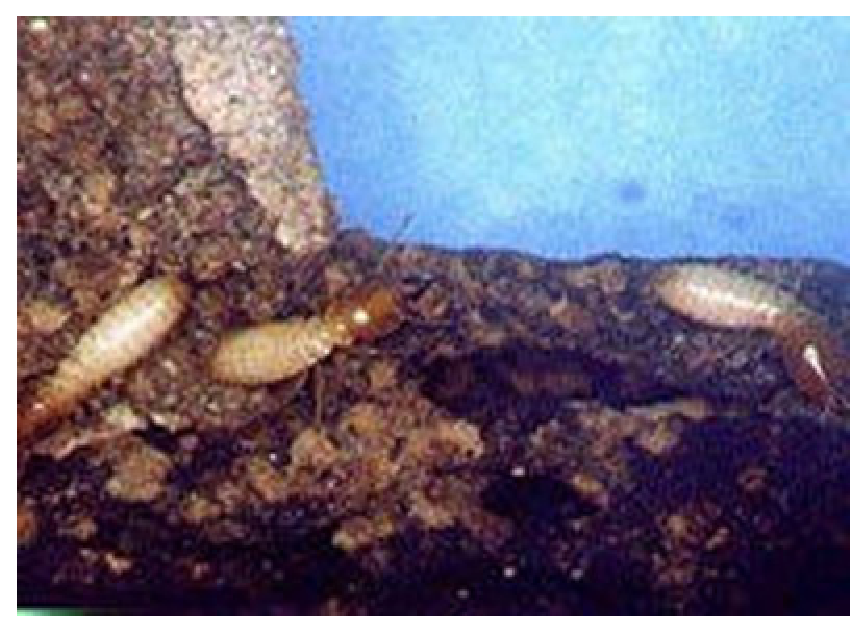
\includegraphics[width=1\textwidth]{Cap1/cupimconcreto}
%\caption{Exemplo real de cupim frente ao seu dilema.}
%\label{FDII}
%\end{figure}

\section{Outline of this work}


